\section{Introduction}
%% High level disaggregation overview, no remote CPU
Disaggregation is an architectural paradigm which separates a computer's
resources from its CPU by a network. While the network provides flexibility it
comes at the cost of additional access latency
-- nowhere is the cost more expensive than between CPU and main memory.
Increased latency only becomes more problematic when disaggregated memory is
shared, and contended for. In a non-disaggregated setting, the memory of a
remote machine is co-located with a CPU which serializes memory accesses, for
example though RPC calls. Such serialization is impossible in the disaggregated
setting as by definition no such remote CPU exists.  This absence causes the
cost of traditional serialization mechanisms, such as locks, to skyrocket when
naively ported to disaggregated memory.

%% contention
Fighting high cost coordination is not a new battle. Entire classes of lockless
data structures were invented to prevent contention unless true data races
exist, allowing for uncontested access to shared structures.
~\cite{simple-fast,lock-free-skip,non-block-binary,read-concur-btree,lock-free-btree}.
Similarly the advent of NUMA servers lead to the production of locality aware
algorithms and data structures which scale to thousands of cores.
~\cite{linux-scale,black-box-numa}\todo{many cites for numa}. The common thread
that ties these two contexts to the concept of disaggregation is that memory
accesses are one-sided (executed directly on memory with no additional
computation), and the latency cost course grained serialization is high.

%dissagregation as an archetecture different from prior work
Disaggregation extends the notion of NUMA to beyond a single machine and into a
new territory of system architecture. The most striking addition to the design
space is the inclusion of high-speed programmable networks. The choice of
networking hardware, in terms of switches, (network interface cards) NICs, and
transports like PCIe have a direct impact on the design of the operating system,
algorithms, and data structures built to run on
them~\cite{dredbox,firebox,machine,legoos,supernic}.  For example Mind used a
programmable switch for address protection, and as a TLB for disaggregated
memory~\cite{mind}.  Programming network devices is difficult work as they are
resource constrained both in terms of general compute and memory, and often lack
high quality developer tools. These development barriers mean that few
algorithms and data structures have been designed with programable network
hardware in mind. Despite the technologies reported benefits, we as a community
lack principles to determine how to integrate programable networks into
disaggregated architectures.

%% lots of work to do, kind of a dead paragraph
%Disaggregation is still in its infancy, and the community of system designers
%currently lacks the tools and concepts which will make it a practical reality.

A litany of prototypes have been built which demonstrate the feasibility of
disaggregation~\cite{infiniswap,fastswap,leap,legoos,aifm,kona,reigons,software-far,lite,semeru}.
However, little conformity has been reached in terms of system design and
expectation. One of the few salient points, is that the cost of coordination is
high, and is therefore often avoided. The few prototypes which do coordinate
accesses to far memory have sophisticated and complex techniques for achieving
serialization~\cite{clover,one-sided-hash,sherman,ford}. Our insight is that nearly all of
the serialization and synchronization issues associated with memory
disaggregation are not new. We have found that many practical approaches can be
mined from prior literature aimed at scaling to many cores, or directly access
the memory of a remote machine. This insight ends where programmable networking
begins, as little prior work (with the exception of PIMM memory~\cite{near-memory-structs}),
includes programmability on the data path.

%% What this paper is not
This paper is focused on data structures for disaggregation, it is not a systems
summary.  Many projects exist which are designed for the disaggregated model,
few of which will be covered in detail. An overview of the state of the art
systems circa 2021 can be found in Yelam~\cite{yelam2022systems}.
%%
To be explicit about scope this is not a paper covering remote paging or caching
systems~\cite{fastswap,kona,infiniswap,leap,legoos}. These systems design their
virtual memory interfaces to incorporate far memory. Each takes into account the
ratio of local to remote memory, and take measures to design their swapping
systems with the cost of accessing far memory in mind.  However, none share data
across processes so their only performance effect from far memory is the size of
their cache, paging policy, and round trip cost. As such each system is
primarily constrained by the access pattern of their programs. We consider
locality optimization to be a single facet of the design space for
disaggregation and address it more fundamentally in
Section~\ref{sec:techniques}. We reference systems only in terms of their data
structure design.
%%
Moreover, this paper is not theory. All data structures investigated within have been
implemented using real hardware. While some papers referenced may be theoretical
in contribution~\cite{flat-combine,hopscotch,linked-list-cas}, they must be
backed by a concrete implementation. As such our scope is limited to data
structures which can be implemented using instructions available on commodity
hardware.

% Paper Goals

The future of resource disaggregation is unclear. Thus far the 20x increase in
latency between local and remote memory has made practical memory disaggregation
a non-starter. Our goal is to take a small step forward by
identifying new and existing design principles for disaggregated memory.
%%
In this paper we survey prior algorithmic and data structure trends driven by
shared memory scalability and ask the question \textit{Which existing techniques
apply to memory disaggregation, and what new techniques are enabling the
technology?} This survey covers concurrent data structures, NUMA data
structures, and RDMA key value stores which make use of one-sided operations.
We then analyse the first few works on disaggregation specific data structures
and identify the techniques used to achieve high performance in the face of
contention. When a project does not make use of an identified technique we
comment on how it may have improved (or reduced) the systems performance. The
final part of our analysis focuses directly on the serialization mechanisms used
in each data structure with respect to how programable networking devices may
accelerate it. In particular we focus on cases where maintaining a small amount
data structure specific state in network can greatly improve operation
throughput and latency.

% Although problems such as the memory wall have been
% cited for over a decade~\cite{blade-server}, and SSD \& HDD disaggregation is
% now commonplace in data centers~\cite{decible}, main memory disaggregation still
% has significant obstacle to overcome before it becomes a practical architecture.
% Local main memory is still 20x faster than remote memory.

% This is no small
% latency factor for engineers and scientists to contend against. Our goal is to
% first identify the ideas that enable practical disaggregation today. To do so we
% provide a brief survey of lock free data structures, multicore and NUMA, RDMA
% Key Value Stores with the context of disaggregation in mind and make note the
% the techniques used to enable scalability, and reduced latency.

% Using this information we break down a set of techniques and describe them more
% generally before applying a more in depth analysis to existing disaggregated
% data structure centric systems. In cases where systems forgot these techniques
% we comment on potential alterations which may improve performance or
% scalability.

% We close with discussion topics such as additional considerations for resource
% disaggregation, the potential pitfalls of far memory design, and the potential
% role of programable networking hardware in the future of disaggregation.

\section{Background}

%Disaggregated Model
Disaggregation is a general term used for the separation of resources by a
network. The composition and topology of the network plays a large role in how a
disaggregated computer will manifest. The disaggregated model we consider most
prevalent is that of the rack-scale computer. In the rack scale design servers
in a rack have a resource role - compute, memory, storage, accelerator. Each
server is connected via a fast network i.e. 100-400Gbps ethernet or above. The
topology of the rack is up for debate, however many suggest that each server is
interconnected with a traditional TOR, or with a special purpose middlebox for
memory traffic~\cite{disandapp}. Proposals for other topologies such as torus
exist, however we scope ourselves to the prior configuration. In the rack scale
model we consider all memory traffic in a rack transits a centralized switch,
and all the traffic for an individual machine flows through that machines NIC.
Figure~\cite{fig:rack-scale} provides a high level overview of this system
architecture.


\begin{figure}
    \begin{centering}
    \includegraphics[width=0.45\textwidth]{fig/rack.pdf}

    \caption{ A rack-scale computer is a single rack of network connected
    machines, each with a specific purpose, compute, memory, or storage. Each
    machine is equipped with a high performance NIC (100Gbps+), interconnected
    with a top of rack switch. Many designs include some degree of
    programmability in the network~\cite{disandapp}.
    }
    \end{centering}
    \label{fig:rack-scale}
\end{figure}

Disaggregation assumes that memory operations, i.e. reads and writes are issued
over the network rather than across a traditional memory bus. RDMA is a popular
networking technology which allows clients to read and write directly to a
servers memory without CPU involvement. RDMA is also known for having high
throughput and low latency. Due to it's direct applicability most memory
disaggregation proposals assume RDMA capable networks as an essential
architectural building block. However, alternative interconnect proposals exist.

GMS~\cite{gms} suggests that global memory be maintained alongside an entire
networking stack. In pure resource disaggregation, no remote CPU's exist which
exempts this approach.  Alternatively, rather than explicit reads and writes
cache coherence algorithms could be used to fetch data from remote memory on
custom interconnects such as in Kona~\cite{kona}.

RDMA is a middle ground. The RDMA specification gives a set of \textit{verbs}
which are memory operations that the NIC can execute. These verbs are similar in
some respects to RPC calls, or simple instructions. As long as an algorithm can
be described using the RDMA calls it can be executed on remote memory. The
advantage to RDMA is that the operations it supports are general. The downside
is that some algorithms are difficult to execute using one sided verbs. The
prototypical example is pointer chasing which requires a round trip for each
resolved pointer.

The research space closest to practical memory disaggregation is RDMA key-value
stores (KVS). The performance expectation for their read and write operations is
typically hardware line rate, or its packet per second limit. Even a few CPU
instructions per packet can drop performance below line rate, so to improve
performance and reduce CPU utilization, key value stores use one sided RDMA
operations. These KVS make careful selection of their data structures for
efficient integration with RDMA~\cite{hopscotch,cuckoo}, and select RDMA
communication protocol (reliable connections, unreliable connections, unreliable
datagrams) which promote the highest performance the current generation of
hardware can offer~\cite{herd,storm}. The direct applicability of prior KVS work
and disaggregation end when two sided approaches like RPC or two sided RDMA are
utilized for serialization. For example, reads can be performed asynchronously
using one sided operations, while writes are serialized by a two sided
operation~\cite{pilaf}. This allows a CPU to perform the locking and execute
multi step critical sections, such as pointer chasing, with low latency.
Unfortunately these hybrid approaches are not available to pure disaggregated
systems.

\todo{Programmable Networking}

\section{Challenges}

The largest challenge in realizing disaggregation is latency. We have arrived at
a point in history where disaggregation has become feasible only due to dramatic
improvements in networking hardware which allow for ultra low latency access to
remote memory. This trend is expected to continue, and the overhead of remote
memory will continue to shrink as a function of network hardware performance.
Even when network hardware technology has peaked, and remote memory is at
it's lowest cost, it will still be much more expensive than a local memory
access due to physical limitations such as the speed of light. In the
expectation of eventual reasonable, but not low cost disaggregated memory access
we focus on the fundamental challenges that will still need to be solved for
general purpose computing. 

The next big challenge is sharing and contention. Disaggregation suffers the
same issues around sharing and contention that any multiprocessor system does,
however the effects are more severe due to increased latency of remote memory.
Naively ported mutual exclusion algorithms like spinlocks incur huge overheads
as each failed attempt to acquire the lock results in an additional round trip.
The holy grail of remote memory operations is an $O(1)$ algorithm for reading
and writing. Each solution in section~\ref{sec:solutions} is an approach to
reduce the number of round trips and thereby get closer to an $O(1)$ common case
read and write.  We focus on techniques to alleviate sharing and contention
latency. These techniques often come with tradeoffs, such as additional
bandwidth, or memory which complicate the evaluation of effective techniques.

\textbf{Mutual Exclusion and Round Trips:} 
%%
Most common techniques for locking
and mutual exclusion scale poorly to disaggregated memory. For instance the
common approach of acquiring a lock, performing work, and then unlocking, is not
expensive when memory is only a few nanoseconds away, but when the lock is in
remote memory each test operation requires a round trip.  Reading, and then
writing to mutually exclusive data requires at least four round trips. The first
to acquire the lock, the second to read the data, another to write an update,
and a final message to unlock.  Amortizing this cost is essential for
disaggregation. The cost can be reduced using patterns common to opportunistic
algorithms. The same operation requires only three round trips by by performing
the read first, then the write, and finally an opportunistic commit operation to
make the write visible to other threads. Typically this will fail if the read
was stale, or another thread concurrently wrote to the data structure. This can
be further improved by amortizing the reads and writes. For instance reads of
shared data can be executed periodically out of band with writes to keep a local
cache up to date.  Writes can be executed with the expectation that the
asynchronously read data is up to date, and the opportunistic commit operation
can be run simultaneously with the write. In the best case this reduces the
observed latency on a write to a single round trip, but it can easily degrade to
many retires if write or read data is contested. 

% Clover follows this last
% pattern closely, and achieves good performance on read heavy workloads, but
% suffers when many writes occur~\cite{clover}.


%Section Pitfalls of some technqiues
\textbf{Centralized Serialization} 
%%
An attentive reader may now ask \textit{If the cost of round trips is so
extreme, why not serialize access to remote memory through centralization?} The
simple answer is that any centralized solution is itself an explicit bottleneck.
The aforementioned Clover shows experimentally that a centralized solution can
only achieve half of the read throughput that their decentralized solution
can~\cite{clover}. Similar prior work on near memory computing showed that using
traditional serialization methods, such as locks, also quickly bottleneck in
comparison to well crafted opportunistic algorithms~\cite{near-memory-structs}.
If this were not the case, a reasonably simple solution for serializing access
to disaggregated memory would be to port existing RPC based approaches like
Herd~\cite{herd} to a SmartNIC on each memory server. As shown in FairNIC and
Ipipe the number of additional cycles that SmartNIC has to process packets is
slim, and any additional work causes a drop in performance~\cite{fairnic}[Figure
2]~\cite{ipipe}[Figure 4]. Because centralized solutions have an inherent
bottleneck utilizing them is a balancing act. Figure~\ref{fig:middlebox_model}
provides an abstract visualization of the tradeoff between centralized
serialization and performance. Some systems may benefit from in network
serialization, while others may falter if the cost or resolving their conflicts
is too high. The cost to resolve conflicts is directly related to underlying
data structures of the system.

\begin{figure}
    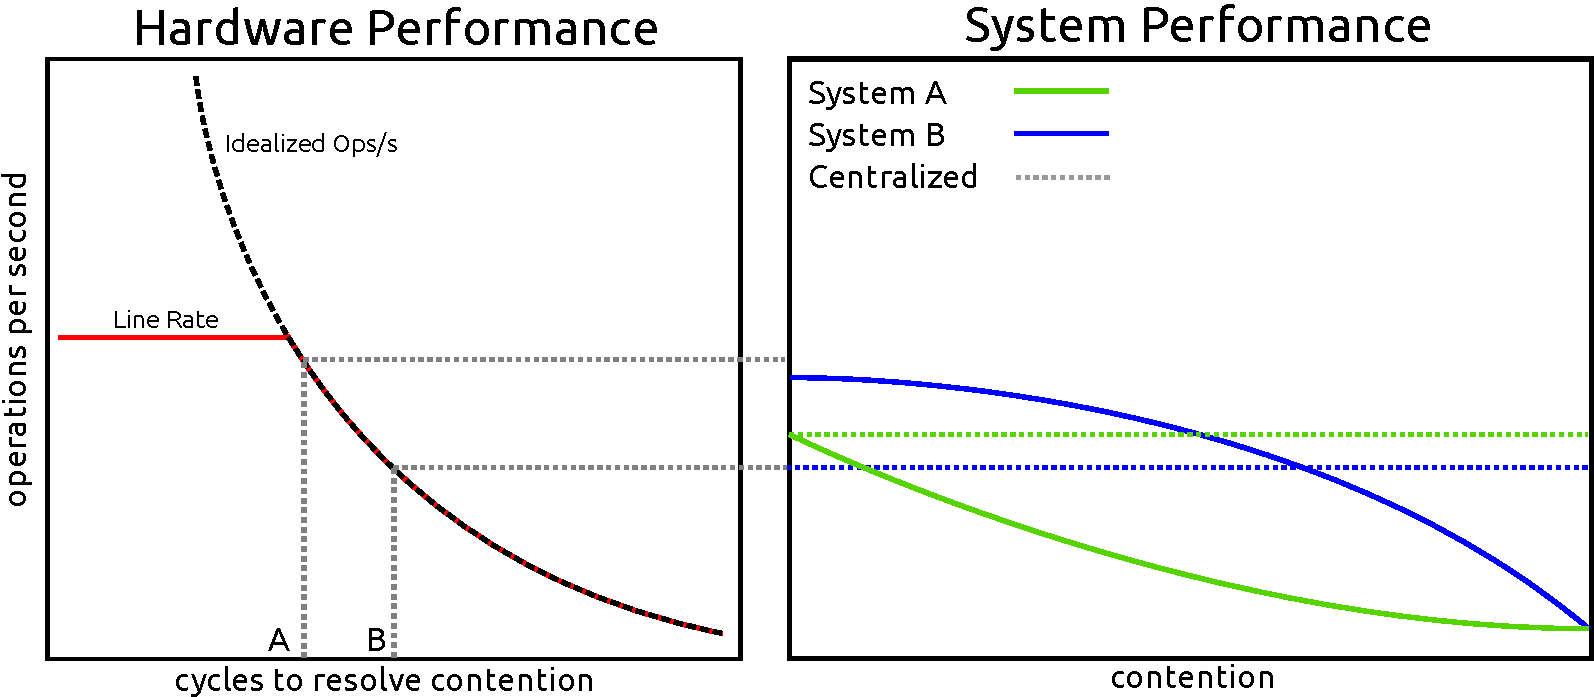
\includegraphics[width=0.48\textwidth]{fig/in_network_tradeoff.pdf}

    \caption{The tradeoff between in network serialization, and end-to-end
    techniques. On the left is a model of of hardware performance vs the work
    required per packet to resolve contention. On the X axis the cost of
    resolving contention in two system A and B are marked. On the right, the
    benefit of applying contention resolution to these systems. System only has
    a benefit as the cost to resolve it's conflicts are below the hardware cost.
    System B loses performance with the centralized solution while contention is
    low.}

    \label{fig:middlebox_model}
\end{figure}

% My approach uses a centralized serialization
% point to alleviate coordination. However it has been shown that doing all the
% work by a centralized core is slower than a carefully crafted concurrent
% solution~\cite{near-memory-structs}. The insight here is that if we have a core
% close to memory it can do things like pointer chasing faster than remote. They
% demonstrate that PIMs are not sufficient to solve far memory problems. But it
% will become bogged down at some point due to being centralized. That's when a
% concurrent algorithm with less contention moves faster. The key thing about this
% centralized point, is that it must have excess space above line rate with which
% to coordinate. For example in we show that there is
% some headroom for processing with x number of cores. This gap is the processing
% gap that we can use to resolve contention.

\textbf{RDMA Atomics}
%%
The RDMA specification includes atomic operations for one-sided serialization.
These operations present their own unique challenges which are discussed here as
RDMA is the primary technology upon which disaggregated systems have been built.
Atomic performance in terms of packets per second is roughly half of read and
write performance for the same sized data. The performance of operations drops
further if the data is contested by many RDMA connections. Reaching the atomic
bottleneck is not common in opportunistic algorithms as the pace of attempted
lock operations is offset by reads and writes~\cite{clover}. In contrast
algorithms that use traditional locking can easily reach this limit, as a
spinlock access requires atomics to be continuously issued until the lock is
acquired. Faster locking operations are possible if the lock is located on
device mapped memory, this prevents each lock request from making two PCIe round
trips. Network devices such as ConnectX series NICs expose this memory to
programmers, but it is limited, and demands that data structure which want to
use it have their memory layout organized accordingly~\cite{sherman}. One final
pitfall of RDMA atomics for locks is that they lack fairness. This can lead to
extreme tail latencies which is not ideal for memory operations.

\section{Solutions}

\begin{table*}[h]
%\begin{table}[h]
    \centering
    \begin{tabular}{ c | c | c | c | c | c | c | c | c }
        & project & \shortstack{read \\ inflation} & \shortstack{relaxed  \\ layout} & \shortstack{pre-\\compute} & \shortstack{optimistic \\ concurrency} & \shortstack{metadata \\ caching} & \shortstack{client \\ coalescing} & \shortstack{self \\ verifing}  \\ \hline
                                                                %N          %R          %P          %O          %M          %C          %W          %S
\multirow{3}{*}{\rotatebox[origin=c]{90}{\shortstack{Multicore \\ NUMA}}} & \shortstack{Flat \\ Combining}~\cite{flat-combine}   & \nullcirc & \nullcirc & \nullcirc & \nullcirc & \nullcirc & \fullcirc & \nullcirc \\ \cdashline{2-9}
         & \shortstack{Hopscotch \\ Hash}~\cite{hopscotch}         & \fullcirc & \nullcirc & \nullcirc & \nullcirc & \nullcirc & \nullcirc & \nullcirc \\ \cdashline{2-9}
%\multirow{1}{*}{\rotatebox[origin=c]{0}{\shortstack{NUMA}}} & \shortstack{Blackbox \\ NUMA}~\cite{black-box-numa}     &  &  &  &  &  &  &  &  \\ \hline \hline %\cline{2-10} \cline{2-10}
        & \shortstack{Blackbox \\ NUMA}~\cite{black-box-numa}     & \halfcirc & \nullcirc & \nullcirc & \fullcirc & \fullcirc & \fullcirc & \nullcirc \\ \hline %\cline{2-10} \cline{2-10}
\multirow{4}{*}{\rotatebox[origin=c]{90}{\shortstack{RDMA \\ Key-Value}}} & pilaf~\cite{pilaf}                                      & \nullcirc & \nullcirc & \nullcirc & \nullcirc & \nullcirc & \nullcirc & \fullcirc \\ \cdashline{2-9}
         & farm~\cite{farm}                                        & \fullcirc & \nullcirc & \nullcirc & \fullcirc & \fullcirc & \fullcirc  & \nullcirc \\ \cdashline{2-9}
         & herd~\cite{herd}                                        & \nullcirc & \nullcirc & \nullcirc & \nullcirc & \nullcirc & \nullcirc  & \nullcirc \\ \cdashline{2-9}
         & cell~\cite{cell}                                        & \nullcirc & \nullcirc & \nullcirc & \halfcirc & \fullcirc & \nullcirc  & \fullcirc \\ \hline \hline
         % & % fasst~\cite{faast}                                      & \nullcirc & \nullcirc & \nullcirc & \nullcirc & \nullcirc %& \nullcirc & \nullcirc \\ \hdashline
         % & % erpc~\cite{erpc}                                        & \nullcirc & \nullcirc & \nullcirc & \nullcirc & \nullcirc & \nullcirc & \nullcirc \\ \hdashline
         %& storm~\cite{storm}                                      &  &  &  &  &  &  &  \\ \cdashline{2-9}
         % & 1RMA~\cite{1rma}                                        &  &  &  &  &  &  &  \\ \hline \hline
\multirow{5}{*}{\rotatebox[origin=c]{90}{\shortstack{\small Disaggregated \\ \small Datastructures }}}        & Clover~\cite{clover}                                    & \nullcirc &  \halfcirc &  \nullcirc & \fullcirc & \fullcirc  & \nullcirc & \nullcirc \\ \cdashline{2-9}
%\multirow{5}{*}{\rotatebox[origin=c]{90}{\shortstack{Far-Memory \\ Structures}}}        & Clover~\cite{clover}                                    & \nullcirc &  \halfcirc &  \nullcirc & \fullcirc & \fullcirc  & \nullcirc & \nullcirc \\ \cdashline{2-9}
         & \shortstack{RACE}~\cite{write-op-hash}            & \fullcirc  & \fullcirc & \halfcirc & \fullcirc & \fullcirc & \nullcirc & \fullcirc \\ \cdashline{2-9}
         & Sherman~\cite{sherman}                            & \fullcirc & \fullcirc & \halfcirc & \fullcirc & \fullcirc & \fullcirc & \fullcirc \\ \cdashline{2-9}
         & Ford~\todo{}                                          &  &  &  &  &  & \\ \cdashline{2-9}
         & Mind~\cite{mind}                                                & \nullcirc & \halfcirc & \halfcirc & \nullcirc & \fullcirc & \nullcirc & \nullcirc \\ \hline


    \end{tabular}

    \caption{Cross section of systems and technqiues. Full circles
    \fullcirc imply that a system uses the category, \halfcirc denotes when a
    system meets the qualification in spirit but not explicitly, and \nullcirc
    when the technique is absent.}
    
    \label{tab:1}
\end{table*}

Reducing round trips requires algorithmic and data structure improvements. A
common tactic to reduce round trips is to reduce the precision required by an
operation. Reduced precision can enable operations to succeed even when they are
executed with stale information. There is always a tradeoff when precision is
reduced, it can incur additional bandwidth, or increase a data structures memory
footprint. Less generalizable strategies take advantage of environment specific
conditions to improve performance, such as resolving conflicts locally when CPUs
are colocated. In this section we overview common techniques used to reduce
round trip times. These techniques are not unique to disaggregated literature.
Work on current data structures, NUMA systems, and RDMA KVS have paved the way
to memory disaggregation. We reference systems which utilize these techniques in
this section, prior to covering each system in detail in
section~\ref{sec:systems}.


\subsection{Read Inflation} \label{sec:readsize}
%%
Writes can be accelerated by reduced the constraints on their location and
expanding reads to capture the sloppy writes. The inflated reads are recomposed
into coherent state locally at the cost of some additional computation. How much
compute is is dependent on the data structure, and overarching operation being
run. As an example consider a sorted list accessed by many processes. Each
insert is expensive if it must be globally coordinated. However it is cheap if
each process maintains its own locally sorted list. A call to \textit{max} which
returns the max globally can peek at the head of each list. The result is a list
of local maxes, from which the global max can be locally computed.  For $n$
processes this inflates the cost of the read by $n$ in bandwidth however it
removes the need for coordination. 

Algorithms like hopscotch hashing~\cite{hopscotch} (used in Farm~\cite{farm})
and Robinhood hashing~\cite{robinhood} are designed to have good cache locality.
Hashed data is stored using open addressing, a layout scheme which allows for
flexible data placement in the hash index.  Both of these hashes specify that
data must be placed within a bounded range of the index the data hashes to. The
range of valid locations is known apriori so a requests are guaranteed to
succeed if they hash the data and perform a read large enough to capture the
entire valid range of the datas indexes.

Data structures with locality invariants are beneficial for disaggregated
systems as their reads can tradeoff bandwidth for round trips. Future
analysis into other cache optimized data structures may be fruitful in finding
new candidate data structures for disaggregation.

\subsection{Relaxed Layout} 

Somewhat ironically while tight locality invariants enable $O(1)$ reads, loose
locality invariants reduce the price of writes. Data structures with strict
semantics such as ordering are difficult to maintain under contention as
potentially many elements must be read, and reorganized to achieve an operation
such as an insert.

For example Sherman~\cite{sherman} uses relaxed ordering in it's B-tree buckets
so that writes can succeed more frequently in $O(1)$. This also has the effect
of reducing write amplification as only a single entry is written, and not an
entire ordered bucket. Similarly One-Sided-Hash~\cite{one-sided-hash} uses
associative cashing and power of two in order to allow for multiple write
locations. By relaxing the structural invariants higher write performance is
achieved. A structures overall performance will be impacted by how data layout
is relaxed. As detailed in the prior section if the layout retains locality
reads can remain $O(1)$ at the cost of bandwidth. If however a relaxed layout
means that a writes location is determined by a traversal of many pointers it
will skewer read performance.

\sg{Techniques which amortize read cost may be benificial for read performance,
for example if reading data the first time requires a high cost, but it becomes
$O(1)$ after being resolved it may be a worthwhile tradeoff. For such tactics to succeed }

\subsection{Precomputation} 

With careful design some data accesses can be optimized by adding computational
work to clients. One example is Clios single level page table~\cite{clio}.
Traditional page tables require a pointer based walk to resolve virtual
addresses. A page table walk is expensive for disaggregated memory as each
levels resolution requires a round trip. Clio achieves an $O(1)$ page table
lookup by pushing the complexity to malloc. The page table is a hash of virtual
addresses, calls to malloc generate candidate virtual addresses until one with
no collisions in the hash is found. This allows for all page table lookups to
occur with a single round trip.

Trading off algorithmic complexity with computation complexity is largely
unexplored territory, fortunately some design pitfalls can be determined with
speculation. Any degree of global churn in a data structure, such as resizing a
hash table will have amplified cost if large amount of precomputation work has
been done to produce the current hash. Here any strategy which preserve the work
will be beneficial in overall system performance. Precomputation should also be
pushed to uncommon tasks, or tasks which are not latency sensitive.
Precomputation in the data path may result in performance losses greater than
the avoided round trips.

\subsection{Optimistic Concurrency} 

Lock based mutual exclusion requires at least two round trips for acquisition
and release. Opportunistic algorithms and lock-free data structures have the
potential to reduce the number of round trips by committing operations with a
single atomic operation, i.e compare-and-swap. There is a deep history of
opportunistic algorithms and data structures. Most common data structures have
an opportunistic implementation for example, linked
lists~\cite{linked-list-cas}, queues~\cite{simple-fast}, skip
lists~\cite{lock-free-skip}, binary trees ~\cite{non-block-binary}, and
b-trees~\cite{read-concur-btree,lock-free-btree}. A comprehensive review of
these structures is beyond the scope of this paper. At a high level the
opportunistic advantage is that in the absence of a true data race, operations
can complete with no blocking, or retries.

The main tradeoff of opportunistic approaches is that they experience high tail
latency under contention, and often lack fairness. These drawbacks are typically
those cited when RDMA systems choose to serialize writes using CPU implemented
RPCs rather than RDMA atomics~\cite{pilaf, cell, herd}. Opportunistic algorithms
have a pragmatic advantage given that current RDMA hardware supports
compare-and-swap, as well as fetch-and-add operations, which are the necessary
building blocks for most opportunistic data structures.

\subsection{Metadata Caching}
\todo{old rewrite}
Shared state is a serious bottleneck for highly parallel systems especially when
the cost of accessing a resource is high. One common pattern is to simply
partition resources so that no sharing is required. For instance systems like
LegoOS~\cite{legoos} and FastSwap~\cite{fastswap} don't support any state
sharing between processes. In multithreaded programs sharing is often an
unavoidable consequence of the work being done. For higher performance processes
can replicate parts of the shared structure and cache the portion locally. In
the case where there is little or no contention this allows processes to make
forward progress without accessing a shared resource. In the disaggregated
setting this is particular important as the cost of accessing remote memory is
particularly high. For instance Clover~\cite{clover} locally caches the metadata
of it's remote database to perform opportunistic writes, and Black Box
Numa~\cite{black-box-numa} maintains a replicated log of every operation. Of
course, when conflicts do occur the benefits of replicating state diminish and
simply become a memory overhead. The choice of replication strategy, and degree
of replication which will result in the highest cost to performance boost is
workload dependent.


\subsection{Client Side Coalescing}
If clients to remote memory are colocated on the same machine local memory can
be used to consolidate conflicts. For example, designating a single core to make
requests reduces the number of conflicts at remote
memory~\cite{flat-combine}~\cite{sherman}. Many disaggregated solutions supposed
rack scale deployment, therefore while structures must accommodate thousands of
threads, requests can be consolidated at the machine or NUMA level, to reduce
round trips caused by failed contended access to remote locations. This
consolidation requires careful consideration. For example funneling all requests
through a single core will result in a bottle neck. Therefore all non-blocking
operations should be made independently. However, locking operations, if
infrequent could see large performance boosts from client side consolidation.

Properties such as fairness are more easily enforced at the client side. For
example queues are simple. This can allow for cluster approximate fairness where
each machine, or numa domain is fair with respect to itself, but not the system
as a whole.

\subsection{Self verifying} RDMA reads and write have a variety of ordering
guarantees depending on the transport used, but in general only operations on
the same queue pair with a reliable connection are ordered with respect to one
another. Accesses to memory from the host CPU only has atomic memory operations
as a tool to order reads and writes with the NIC. This leads to read tearing
where either the host CPU, or a client RDMA request sees a partially completed
write. In the absence of serialization the data itself can be made self
verifying.  Pilaf, and Cell are notable examples of KV stores which use self
verifying data~\cite{pilaf,cell}. Self verifying data comes in a variety of
forms. The most common is the inclusion of a checksum, typically a CRC along
with the data. If a write is partially completed a client can detect the
inconsistency by computing the checksum. This adds CPU cost for the sake of
concurrency. For transactional operations which require multiple independent reads
to be consistent version numbers are used. If at the end of an operation the
version numbers of each read do not match, the read is aborted.


\section{Lesser Remote Memory Techniques}
\label{sec:additional}

\todo{This section is extremely rough}

Section~\ref{sec:techniques} describes the top seven techniques we found to be
most used, and effective in our literature survey. However there are many more
common considerations which we briefly detail here.

\subsection{Network Caching} A variety of caching techniques reduce latency for far memory
application. Caching allows for a two fold benefit. The first is that the
distance between requests and the required data is less. Caching on a switch
removes the last hop in a rack, and on a NIC removes a PCIe round trip. The
dangers with caching is that the important caching data must be determined
somehow. Traditional caching techniques can lead to massive bandwidth inflation.
The second advantage of caching in network is centralization which can reduce
the communication between hosts.

\subsection{Memory Traffic} As noted during Yizhous research exam. There is a
potential for a massive amount of additional traffic to flow over the network
due to accessing memory. There are various factors for this. In paging and cache
based transparent systems~\cite{fastswap,kona,gms,infiniswap,legoos,lite}, the
size and associativity of the local cache determines the traffic rate. Each
traffic rate is also a function of the programs memory access policy, and the
systems eviction policy. Shrinking a local cache could significantly inflate
traffic. This is simultaneously true for any cache coherence protocol, or data
structure which needs to have a locally up to date version of remote data prior
to making an update. Memory traffic can be deflated by using traffic agnostic
techniques such as compression, or by modifying the access policy, such as
prefetching more or less remote memory. There is no magic bullet for this
problem, each instance of a remote memory system will have to solve this problem
in its own way.

One aspect of caching protocols is that they explode the traffic requirements.
On memory busses only intended for memory traffic, this may be acceptable, but
on an RDMA network it's going to be most of the traffic. For example the
proposals in Thinking outside of the Box~\cite{design-far-memory-struct} calls
for cache coherence protocols, while Mind~\cite{mind} actually implements one.
Swordbox actually removes the need for the cache coherence by fixing the missing
data in network.

\subsection{Write amplification mitigation}
\label{sec:write-amplification}
%%
Remote structures sometimes require write
amplification. Consider a set of entries each guarded with a checksum for
integrity. An update to any entry requires the recomputation of the checksum,
and the rewrite of the continuous addresses in order to make the write in a
single round trip. Depending on the bucket size of the entries the write can
grow arbitrarily. Another technique is to make each entry have it's own checksum
for it's integrity, and to only update the bucket checksum when all items become
static.

\subsection{Network Serialization} 
\label{sec:net_ser}
%
centralized in network compute can be used to steer and modify
requests when data races and conflicts occur. The downside is that this takes an
extra bit of in network processing, but it gets a big speed up. In order for a
middlebox to make the correct steering decision it requires all of the
information necessary to preserve the data invariants of the structure it is
steering into. This limitation demands that the data structure itself be well
conditioned for this property, and be able to deal with potential variance in
its structure.

A potential use for steering is also to perform in place updates while allowing
for reads. For example imagine updating a range on a data structure [x,y] the
first step of the operation could be to lock the region, then copy [x,y] to a
new location [x',y']. During the update reads are steered to the new [x',y'] and
the update is made in place on the old [x,y]. When the operation is complete the
steering stops and the update is atomically visible. This could be useful for
non-pointer based structures like hopscotch hashes~\cite{hopscotch}.


Introduce the remote memory techniques at a high level with small examples for each

\section{Systems}
\label{sec:systems}
\todo{rewrite}
In terms of system design the works mentioned in Section~\ref{sec:not}, are
doubtlessly influential on the state of disaggregation. Here we are focus on the
algorithmic material. In particular disaggregated and remote memory systems make
use of the concurrency patterns in lockless data structures. Locking typically
costs two round trips to remote memory, and course grained locking can cause
many processes to block. Many lock free data structures use CAS operations for
serialization, which are implemented as part of the Infiniband RDMA
specification.

\subsection{Lock Free Data Structures}

Huge amount of prior work has been done in developing lock free data structures.
Such structures allow for concurrent reads and writes so a shared structure by
many processes. Rather than modifying a structure by gaining exclusive access,
lock free typically perform work out of place, and then commit the updates to a
structure using atomic operations such as Fetch-and-Add (FAA) and CAS
(Compare-And-Swap). These lockless structures are often opportunistic, and in
the face of contention cause updates to retry multiple times until they meet the
criteria for the update to succeed. Concurrent data structures are useful in
memory disaggregation where the cost of acquiring a lock is orders of magnitude
higher than local memory. If a lockless operation such as CAS is sufficient to
modify a shared structure it avoids the cost of explicit synchronization. Here
we describe a few influential concurrent data structures who's concurrent
techniques are common in disaggregated systems.

Concurrent queues are one of the most simple and intuitive lock free data
structures, with early implementations appearing in the early
90s~\cite{simple-fast}. This algorithm presents a safe way to implement enqueue
dequeue with CAS. The pattern for enqueue is to write out new data, search
concurrently for the tail, and then attempt a CAS to connect the new element. If
failure occurs because a concurrent process wrote to the tail, the CAS fails,
and the procedure retires the traversal until success. This pattern of write
first, commit after is common among concurrent algorithms.

Fomitchev et.al introduces lock free linked lists and skip
lists~\cite{lock-free-skip}. Similar to queues this algorithm allocates tiers of
a skiplist and then incrementally commits them via CAS. This technique requires
additional care as the data structures are more complex, and updates cannot be
committed in a single CAS operation. To solve this problem CAS's are used to
first invalidate nodes, similar to locking, and then updates are applied via CAS
to include new nodes in the skiplist. This work also introduces safety
optimizations such as pointing deleted nodes in lists back to their previous
node to keep the structure valid while the update occurs.

The first instance of non-blocking binary trees was introduced by Ellen et al.
Binary trees represent a far more complex structure to manage concurrently than
linked lists. During insertions BST rotations require multiple pointer updates,
CAS operations can typically, due to spacial constraints, only update a single
pointer per instruction. This leads to a variety of complex corner cases which
leave the BST in invalid states during rotations which can occur per insertion
and deletion. To prevent invalid states non-blocking BST's introduce complex
intermediate states which are designed to route concurrent processes to the
correct locations during updates. These structures take many CAS and write
operations to complete in order to achieve the non-blocking property. In the
space of resource disaggregation O(1) operations are ideal, intricate and
complex pointer structures care both prone to error, and cause many round trips
to traverse. A lesson from non-blocking BST is that the complexity of
non-blocking structures grows quickly as it's invariants become more complex,
and they are not clear cut candidates for porting to the disaggregated setting.

\sg{Various read concurrent, and lock free implementations of B-Tree's have been
developed over the past decade~\cite{read-concur-btree,lock-free-btree}.}
\todo{finish btree}

\subsection{Multicore and NUMA}

\textbf{Flat Combining~\cite{flat-combine}} Locks and CAS are expensive in their
own right, when highly contested the real cost of using either mechanism can
explode as cache protocols, and fairness skew can dominate access costs and
inflate tail latencies. Flat combining dynamically creates a leader for each
access to a critical section. The leader performs the work of all concurrent
requesters in a serialized fashion and notifies them upon completion. This
technique is extremely powerful and is used in NUMA
algorithms~\cite{black-box-numa} as well as RDMA~\cite{flock}. The key insight
here is that the expense of a critical section can be amortized significantly if
is executed within the local confines of a leader, this simultaneously allows
for batching. Individual cores may not be able to push the request limit of RDMA
(7 cores for 8byte 120MOPS on CX5), however on any particular algorithm they
may. In these cases batching will improve performance. For instance 
Clover~\cite{clover} a disaggregated key-value store described in detail later
on, would see a significant performance boost if it applied flat combining if
and when its clients were co-located. This benifit is showcased in a recent
disaggregated B-tree Sherman~\cite{sherman}, discussed later in detail as well.

\textbf{Hopscotch Hashing~\cite{hopscotch}} introduces a cache optimized
hashmap. Similar to cuckoo hashing it is open addressed. When data collisions
occur on inserts, the algorithm searches for a location by looking for a spot a
bounded distance away from the hash location. If an empty spot is found the
value is written, and a marker is written to the original hash location to
inform readers that there is a value $n$ steps away which collided. If no spot
is found for the write, the \textit{hopscotch} is invoked and the procedure for
finding a candidate write is performed iteratively on neighboring buckets until
a new spot within range is found for the new write. If too many hops are taken,
the hash doubles in side and all items are rehashed.

This algorithm was designed to be cache efficient, as lookups would likely be on
the same cache line. It has the additional advantage that when a value is
written, it's location is deterministic within a bound. In remote memory this
allows for $O(1)$ lookups as the size of the read can be expanded to included
the max distance an entry is from its starting location. This structure is
unfortunate in that writes can take many round trips and complex locking due to
the number of rewrites when the hopscotch algorithm is invoked.


\textbf{Blackbox Numa~\cite{black-box-numa}} proposes node replication, a
universal construction for NUMA architectures. Node replication is a generic
formula for transforming any data structure into a concurrent NUMA aware data
structure. The transformation uses a shared operational log which provides
linearizability for all operations to the shared structure. When process runs an
operation, for example an insert into a tree, the arguments of the operation are
appended to the shared log. The log of operations can then be replayed by any
processes to obtain an up to date version of the structure.

Node replication makes use of many optimizations, as the name suggests, the
shared log is replicated on each node. Local copies of the shared structure are
used for queries and to prepare for future operations. Processes on a node are
grouped together, and for performance operations are coalesced and only issued
by a node leader determined by the flat combining algorithm~\cite{flat-combine}.
The shared log is built by appending to it's tail using CAS operations from the
leader of each node. If the leader is behind is scans the list, and attempts to
append only once it's found the tail.

Node Replication takes into account many design considerations which are present
in the disaggregated context. First it assumes a share, and contested region of
memory. Second it assumes that this memory is expensive to access, and that
obtaining exclusive locks is cumbersome. Finally it makes locality aware
decisions when possible for performance. Where the parallel breaks down is that
reads are considered to be essentially free, which is not the case when they
incur a round trip. However this is likely because node replications reads are
bounded cache line size. Due to the linear layout of its log, if it were ported
to far memory a single large read could capture many log entries reducing the
round trip cost.  Another difference is that atomic operations like CAS are
considered cheap, which is not necessarily the case in RDMA
deployments~\cite{design-guidelines}, see Section~\ref{sec:pitfalls} for more
details. 


\subsection{RDMA key-value stores} 
\textbf{Pilaf~\cite{pilaf}} uses just such a mixture of one and two sided RDMA
operations. The key insight is that if a data structure is architects carefully,
the reads can be performed fully asynchronously by one sided RDMA reads which
dramatically reduces server side CPU usage and request latency. This technique
is common in concurrent algorithms, and is readily applicable here. One new
technique for remote memory structures which pilaf introduces is self verifying
data entries. These entries prevent data corruption during races. Incomplete
writes read by RDMA operations can be invalidated by the client. This is one
example of pushing the complexity of a data structure to the client side. Pilaf
does not extend to the disaggregated context directly as writes are handled by a
server side cpu which serializes requests, and processes CRC's. Their rational
is that client side atomic operations are slow, and brittle. 


\todo{Write more about farm as it ticks a lot of the boxes}
%%
\textbf{Farm~\cite{farm}}, similar to pilaf allows for async RDMA reads, and
uses one sided writes. In this way FARM makes use of an entirely disaggregated
applicable algorithm with respect to it's RDMA circle buffers. 
%%
However the writes are made to a buffer which is polled by a server side CPU and
later processed as a transaction. This technique in some ways is a
disaggregation applicable approach. At least the writes side of the rx wheel
uses disaggregated techniques. Senders cache a local copy of the buffers head
location, in the disaggregated world this pointer would need to be updated in a
one sided fashion, in FARM the receiver occasionally sends the new pointer
location back to the sender when more space has been freed up.
Farm multiplexes queue pairs to reduce the strain on client side NIC memory.
While this is not an explicit use of flat combining it does serialize writes on
the client as an optimization.

Farm makes use of lock free operations by applying version numbers to each
transaction item. When async reads come in, they check the version number of the
data, if the version is old, they retry with a random backoff. Writers apply CAS
operations locally to the version numbers asynchronously from the readers.
However as half of it's structures manipulation requires server side processing
it is not directly applicable. The hash table Farm uses is applicable. They use
Hopscotch Hashing~\cite{hopscotch} which places data near keys. This allows a
single read to get the values it needs with a single round trip (as opposed to
cuckoo hashing). This pushes the complexity to the client. To my knowledge this
if the first instance of pushing read complexity to the client in any paper by
inflating the size of the read.


\textbf{Herd~\cite{herd}} improves upon both FaRM and Pilaf in terms of raw
performance by looking closely at the RDMA specific behavior of KV stores. It
considers the hash algorithm carefully to bound the number of one sided reads.
And uses RDMA writes from server, rather than two sided operations to improve
latency. Herds biggest contribution is that it closely analyses RDMA performance
and choses the verb architecture closely. Herd does not apply greatly to
disaggregated contexts as is fully assumes server side CPUs. However, it's one
sided benchmarks are valid and valuable for disaggregated designers.

\sg{Herd is the closest an RDMA key value store gets to being an influence on
disaggregation without crossing the line. I think it might not belong here,
however it takes every other aspect of RDMA performance and remote memory into
consideration. I can imagine a HERD built with NIC's that would meet the
disaggregated model easily.}

\textbf{Cell~\cite{cell}} Investigates the optimal interplay of async client
side requests and server side processing by developing a novel B-Tree structure.
In cell clients perform reads, while the server does the work to process writes
similar to Pilaf.
%
Servers carefully apply locks to internal B-tree nodes to ensure that concurrent
client traversals of the tree are always valid. Clients cache the trees upper
level metadata including key ranges of meganodes (small partitions of the
btree), and the depth of the trees.
%
Keys are protected in two ways, firstly ranges are projected by version numbers.
The version numbers ensure that the root node is the same as the version applied
to the write, two version updates are appled per write so that a concurrent
client can detect a partially complete write. Additionally keys are projected by
a CRC the same is in Pilaf to prevent read/write tearing.
%
Client side traversals of the B-Tree are poor, taking up to 5 RTT to complete
the traversal of the meganodes. They justify their choice by stating that RDMA
is fast. These operations create significant latency spikes for operations, and
inflate bandwidth costs.
%
Cell makes use of opportunistic reads, that is that it assumes that the state of
the tree is readable when reads are attempted, if the server has some subset of
the tree locked during read traversal, the client fails and then retries. This
is true when version, and CRC values are invalid. Cell is not entirely
opportunistic or lock free as on the sever side locks are attained and
serialized in the traditional way. However the techniques of opportunistic
concurrency, i.e. ensuring that each operation keeps the structure in a
consistent state are used by Cell.



%\textbf{fasst~\cite{faast}[\textcolor{red}{x}]} Fasst is Anujs first cut at RPC.
%Similar to ERPC below, FASST argues heavily for the use of two sided verbs to
%reduce the cost of reading. While this makes sense it's not super applicable.
%Many of the observations are around batching, RDMA reliability, and scheduling.

%\textbf{erpc~\cite{erpc}[\textcolor{red}{x}]} Erpc focues on common case RPC
%operations, aiming to reduce drops, avoid pfc, and achieve 100MOPS. This is
%almost entirely RDMA optimization. They note that using connections, the
%scalability suffers. Around 4000 connections the read rate starts to drop.
%Unfortunatly many of the implements for scaling such ad the RPC credit system
%rely on server side participation. ERPC is therefore not a good source of info
%for this RE.


% \textbf{storm~\cite{storm}} Storm makes the argument that modern NICs have the
% ability to scale well, in contrast to what has been stated in prior work. STORM
% uses a hybrid of one sided operations, and two sided operations. To remove the
% cost of pointer chaising, they swap between one sided reads/writes to RPC when
% pointers need to be chased. This approach does not directly port to
% disaggregation, as their are no memory side CPU's to perform the RPC, however
% some of this functionality could be ported to network hardware such as memory side
% smartnics.


% \textbf{1RMA~\cite{1rma}}

% 1RMA argues that the benefits of one sided reads are sufficient enough to
% integrate into large scale production environments, even with their increased
% complexity. 1RMA does not use pure RDMA, and instead exposes an RDMA like
% interface in the kernel networking stack. They take the extreme stance that all functionality which can not be implemented entirely without the aid of software, should be entirely implemented in software, such as connection state, and packet ordering. Whats left is RDMA like primitives which are exposed to the user at a software level.

% Reading through the 1RMA paper~\cite{1rma}, they make the case for basically
% using the NIC to execute remote operations and nothing else. In some respects I
% def get this aspect of the RDMA construction. Push all of the connection
% management to the client side, and just let the RDMA do it's thing with the
% extremely high assumption that the packets are going to make it back with a
% response. By managing everything on the client side we can get things like
% control flow windows, ordering ect without pushing any of this to the hardware
% itself. I think that this set of features is somewhat desirable. It would be
% cool if the NICs could basically just work on ethernet packets, and then if we
% wanted we could interpose on the application level info whenever we wanted.
% \todo{}


%currently just a jotting area for ideas.


\subsection{Disaggregated Systems}

\textbf{Clover~\cite{clover}}
%%
is a key value store designed for persistent, disaggregated memory. All
of it's remote memory operations are performed via one side RDMA, with the
exception of two sided metadata operations sent to non-disaggregated metadata
servers. This architecture is reached by an empirical evaluation of 4
alternative systems, one which uses a centralized coordinator, and another with
no metadata server at all. The out of band approach is found to perform well for
read only, and sparse write workloads. 

Clover makes use of many techniques for optimizing access to remote memory.
Firstly, it's core algorithm relies on optimistic concurrency. Each key in it's
key value store maintains a history in the form of a linked list. Writes append
values to the list by writing to a partitioned address space first, and then
linking the new write to the list via a CAS operation. The CAS location at the
tail of the list becomes stale if contended with another successful write, in
which case a clover client must traverse the list, each key resolution requires
another round trip. To reduce the number of stale requests, the tail location of
each key is cached locally, and periodically updated lazily from the metadata
server. Clover's key-value store has no predetermined or canonical layout, while
this is not necessarily a relaxed layout, the use of a partitioned address space
for writes is a clever way to reduce write conflicts.

%%\textbf{opprotunities}
Clover does not make use of self verifying data
structures, with the exception of it's pDPM direct. Clover writes take two round
trips in the common case, the first to write, the second to CAS. This ensure the
write completes prior to committing with a CAS. Were clover to have a self
verifying write, the CAS could be batched with the write, thereby allowing
partially written writes to be included in the chain in one RTT. Clover assumes
the worst case for clients in which none are co-resident on the same machine. In
practice clover could gain significant benefits by coalescing client writes with
techniques such as flat combining, when clients are co-resident. This
speculation is based on the analysis that Clovers write throughput under 50/50
read write is well below the throughput of a single queue
pair~\cite{design-guidelines}. It could likely gain performance boosts similar
to Sherman~\cite{sherman}, by taking this optimizations into account. 

Clovers data layout is sparse so it cannot simply inflate it's reads in order to
gain more information, and skip round trips. Figure~\ref{fig:clover_alt} shows
clovers memory layout on the left, in which process isolated memory references
each other via pointers. On the right an alternative design shows a similar
structure which allows for traversals using fewer round trips as the size of the
read can be expanded linearly to capture more of the pointers. Note however that
this layout is not identical as reads have no explicit way of determining that a
value has become invalid by reading the data itself. This example is intended to
illustrate an alternative approach which could accelerate clovers pointer
chaining, potentially reducing the requirement for a metadata store. More design
rigor would be required to achieve the same read semantics.


\begin{figure}
    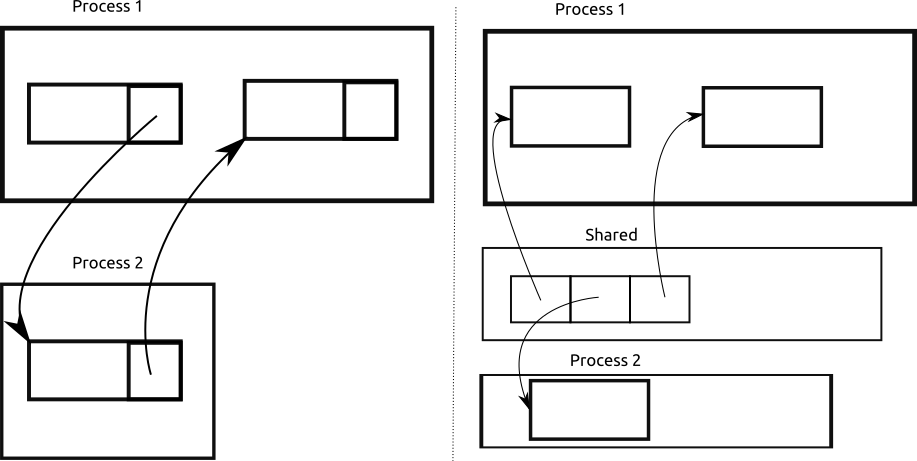
\includegraphics[width=0.45\textwidth]{fig/clover_alt.pdf}

    \caption{An alternative data layout for Clovers key value store, which would
    allow for expanded reads to quickly resolve tails.}

    \label{fig:clover_alt}
\end{figure}


\textbf{RACE~\cite{one-sided-hash}}
%%
designes an RDMA optimized key-value store for remote memory. RACE is
lock-free and makes use of additional memory to reduce conflicts and contention.
RACE notes that prior hash solutions can incur multiple round trips when the
lookups fail, and that if the index must shuffle data such as cuckoo and
hopscotch hashing, lock contention is inflated. RACE caches client metadata
locally to avoid performing directory lookups in the common case. This is a
critical design point as RACE makes use of a two level directory which changes
each time the hash table expands. The local client cache allows for O(1) lookups
by examining the metadata on the client, and only traversing the true directory
when version numbers have changed.

RACE introduces a sophisticated disaggregation specific suitable structure. At
every point in it's design this subtable makes use of RDMA's ability to read
ranges of sequential addresses easily. Firstly all of the buckets in the hash
table are associate so that up to four collisions can occur in a single per read
location. Second an overflow bucket is used as a buffer between each second
bucket. In this way there is additional space for overflow. Finally power of two
is used to select multiple locations for a write to land. In total this forces
reads to read two bucket locations, and two overflow location per read. With an
associativity of 4. In total this gives an extremely high likelihood of $O(1)$
reads while coming at a cost of 16x the read bandwidth. This read inflation is
amortized by only performing two reads, and batching them together
asynchronously. While this reduces the overall load on keys, is half's the
theoretical reads per second due to the packet processing ability of the
receiving side NIC. 

To enable scalability RACE uses concurrent lockless reads and inserts to improve
average case performance.  RACE's main downside is it's inability to reduce the
number of round trips for each operation. Each read requires an access to the
index structure followed by a data read. These two round trips require three
packets. Insertions require four round trips, writes three, and deletions 3.
While batching is used to reduce the cost of round trips when possible the
overall cost remains high especially as the number of RTT leads to high tail
latencies. The requirement for round trips is that it's metadata is divorced
from it's data. Therefore all requests must first make a metadata traversal.
Were RACE to adopt an implicit data invalidation scheme like Clover it could
potentially optimize for one less round trip per read and write.

A short example of an optimization, similar to clover would be to include some
sort of version in the slot, perhaps by removing the fingerprint, or size of
read, or to treat the address of the slot as a version number. Updates to this
key could be done in fewer round trips by trying an opportunistic CAS on the
version number of the slot. With client side search could be avoided and
deletion could be done in a single round trip in the common case where reads are
heavy.

\sg{while reading I think I found a linearizability bug in RACE, I think it's
possible to read invalid data via \textbf{race} condition}


\textbf{Sherman B-Tree~\cite{sherman}}
%%
is a complete implementation of a B-Tree for remote memory.
It makes use of many optimizations for remote memory, including some techniques
not explicitly included in our high level comparison of techniques. Sherman
makes use of optimistic concurrency in order to implement locks. While they
acknowledge that their locking is potentially slow, they make two key
optimizations. Firstly they place course grained locks onto NIC device memory,
this optimization tipples their theoretical throughput. Second they use two
tiers of locking, the aforementioned NIC locks are global, and protect writes to the
entire tree. Local lock tables are implemented on clients in a flat combining
fashion to reduce contention on the server side, and allow for local degrees of
fairness.

Reads are totally async and use entry level version numbers to validate
themselves. Lookups can fail frequently, and the remedy is to retry. For
instance overlapping reads and writes will lead to a retry. Range query are
complex in that they do no contain consistent values. For transactional reads to
occur reads must also lock. This is a strict lessening of constancy which may
not be desireable for future applications.

\textbf{Ford~\cite{ford}}
%%
(This paper is obviously relevant, but the preprint is not out yet. Yizhou is
going to work with them and may get me a copy prior to the RE deadline.)

\subsection{Network Centralized Dissagregation}

\textbf{MIND~\cite{mind}}
%%
differs from other remote memory systems in that it uses the network as a
centralized location to serialize access to disaggregated memory. Mind acts as an
MMU providing isolation and protection to processes running on endhosts. It us  
It makes use of the MSI cache coherence protocol (Modified, Shared, Invalid)
which essentially acts as read/write locks on the memory. Shared means that many
processes can read shared memory, modified means that it's dirty and owned by a
single process, invalid means it's not present. Mind provides both memory
protection and cache coherence. 

As MIND is in-network it's constraints differ from all prior systems in that
serialization is relatively cheap, but state is extremely expensive. In this way
it's only cousin in this work is Sherman, as they both require careful use of in
network locks. MIND uses a sophisticated page table splitting algorithm, similar
to dynamic huge pages which uses minimal memory while providing protection to a
large space of virtual addresses. MIND does share some characteristics with
prior work, in that due to constraints it relaxes the definitions of it's
structures, such as the virtual memory space of remote memory itself, which it
combines into a single contiguous address space. This allows mind to only keep a
translation entry for each memory server it manages.


\section{Future Work Middlebox Incorporation}

The increased gap between computational resources and memory in the
disaggregated model leads to poor performance in some cases. The most blatant is
serialization on contended resources. As noted in Sherman, Clover, Conscious
Hashing~\cite{sherman,clover,one-sided-hash}, writes must be carefully
coordinated to avoid collisions. Fast serialization can be achieved using a
centralized source such as programable hardware in the network. This hardware
performs serialization at the physical level, and is able to process millions of
requests per second. Netlock~\cite{netlock} demonstrates that a switch can
provide centralized locking for millions of requests per second. Mind,
demonstrates that memory protection and cache coherence can be maintained by a
switch~\cite{mind}, and NetChain demonstrated that a set of switches can be used
to obtain millions of consensus operations per second. There are countless works
on in network acceleration for a variety of tasks~\todo{ipipe,netcache,itterally all the things}.

Including a middlebox into the architectural design of a disaggregated system is
a common pattern~\cite{disandapp}. In this model a centralized network device
provides some memory services to the application such as memory protection. The
performance benefit from serialization makes network devices tempting as a key
component of disaggregated systems especially with the proliferation of
programmable networking platforms such as Barefoot Tofino~\cite{tofino3} and
Corundum~\cite{corundum} make developing such software more accessible than ever.

However there is a sweet spot in terms of utility with programable network
devices, Figure~\ref{fig:middlebox_model} shows a general model for network hardware
performance as it does more work per packet. If the work necessary from a
middlebox is higher than a specific number of cycles per packet, then the
overall performance drops below the beneficial range. It has been show in
simulations for PIM architectures that a centralized serialization point for
operations like pointer chasing can slow down operations compared to well
designed data structures for concurrency~\todo{pim Irina citation}.

Therefore the choice of network computation is a balancing act for resource
disaggregation. The balancing act is not only in the choice of \textit{what?}
computation to perform in network, but how the computation should be structured.
Deferring all locking operations to a switch for instance dominates it's spare
resources. If the algorithm making use of switch implemented locks could instead
be implemented using a concurrent algorithm which only makes use of CAS
operations. This would be a fine candidate for RDMA primitives which could
alleviate resource pressure on the switch.

This principle leads to a very simple design guideline for memory
disaggregation. \textbf{Implement all far memory structures with the fewest
constraints possible}. End-to-end approaches should be able to achieve their
operations in O(1) in the common case as round trips are the greatest enemy of
performance.  Clients will benefit from caching data, and performing additional
computation rather than making additional remote requests. Examples include
relaxing data structure invariants such as ordering and placement. Further
networks are fast, and have high bandwidths, if necessary performing larger
reads to obtain correct data is a better decision than making many round trips
to perform a write. If data is truly contested i.e locks, and hot keys,
\textbf{middleboxes such as switches and NICs can provide fast serialization}.
Less is more when leveraging a network device. Algorithms and data structures
leveraging middlebox should be specially tuned to reduce middlebox state. Ideal
data structures would have structural invariants which a middlebox can maintain
while only keeping a small fraction of the data structures information in
memory. Lastly the work done by the middlebox should be minimal. Complex
operations are not ideal for hardware designed to forward packets. Algorithms
with operations that can be satisfied by swapping out values in packets are
ideal. As an example changing the location of a read or write, changing the side
of a read or write, or setting a value in the packets payload. As demonstrated
in SwordBox~\cite{Grant2021InContRes} contention can be avoided in append only
link lists by caching the location of the tail of the list.


Consider how Sherman might be improved by small amounts of application specific
caching on a middlebox. Firstly, Shermans search step has two potential
destinations due to their power of two load balancing. This demands the use of
two packets for each search, an operation required in each operation. A
middlebox can easily reduce this requirement to one packet per read by keeping a
single bit per key which denotes which hash the key used. When the packet
arrives the switch performs the hash, and if the packet is sent to the wrong
destination it steers it to the correct one. As this only requires one bit per
key and cuts the packets per second by half, it would likely be a beneficial
optimization. Further each read requires two round trips. This could be reduced
to one for hot keys. The middlebox could maintain a cache of hot keys (top n),
when a search packet is found, if the key gets a hit, the read is transformed in
location and size to the destination address of the true read. For hot keys this
requires 48 bits per key given Shermans addressing scheme.


\section{Conclusion}

% \section{Snoeren Feedback + general todo}

% \begin{itemize}
    
%     \item break the research exam into a structure with key parts. Alex
%     suggested (systems, challenges, solutions) - I think that the correct order
%     is going to be (Challenges, Systems, Solutions). The reason is that we can
%     break up the parts such as round trips, serialization, and write inflation,
%     discuss the systems and some of their mitigation, then introduce the
%     generalized solutions.

%     \item Learn how to hyphenate correctly. Alexes lesson one-sided operations.
%     One and sided are both adjectives, is it one operations, is it sided. The
%     answer is sided, so one and sided are hyphenated. Actually learn this.

%     \item Naked this - This is reason why we must do $X$. v.s High Tail Latency
%     is the reason we must do x.

%     \item it's vs its. I know the difference, I think I just make this mistake
%     while I'm writing.

%     \item Alex notes, strikes mean remove, circles mean wtf, added punctuation
%     means add punctuation.

%     \item add serialization early in the document so that it's listed as a key problem
%     \item merge the first three sections intro + what this paper is + what it is not into a single section. 
    

% \end{itemize}

% Disaggregated algorithms have the trait that they are one sided, and computed
% over a network.  All shared memory algorithms are one sided, but few are
% designed to scale for hundreds of cores. Often this leads to bottlenecks around
% shared objects such as locks~\cite{linux-scale}. Any shared memory algorithm or
% technique designed to scale is likely applicable to the disaggregated space.

% Therefore the starting place for the history of this exam is concurrency
% algorithms. NUMA systems take care to address the asymmetry of memory accesses
% and divide operations into local and remote. This asymmetry exists in the
% disaggregated context as well. However rather than any piece of data having a
% \textit{local} master, all true data is remote. NUMA systems which allow
% multiple remote accesses to the same data share this quality, and thus their
% techniques are applicable. NUMA which defers to a local core for remote requests
% does not apply here.

% \section{notes}

% The papers~\cite{one-sided-hash} and ~\cite{write-op-hash} are almost
% identical. It's the same author, I'm just noting that the change between NUMA
% and Far memory could use this as a case study.

% Similar to the concept of a bandwidth delay product, in terms of remote memory
% there is a latency operation product which is expanded by the time it takes for
% an operation to complete. For example O(1) will have less active operations than
% an O(2) data structure simply by the nature of the operations. Anything requiring
% a read and a write to complete will take longer to complete due to the round
% trip.

% In the few concurrent papers I read there is the concept of performing a marking
% on a data structure. For example this concurrent binary
% tree~\cite{fast-concurrent-bin} marks edges to ensure that they do not get
% modified in a way that breaks the tree. This marking is similar to placing a
% lock. I think that similar to marking, there should be a way to check a data
% structures in flight operations, if all the operations are known ahead of time,
% and then serialize the requests based on that.

% There is a good argument for algorithms between the two worlds of remote memory.
% On one hand we have pure remote memory, one sided operations with zero
% interference. These are unbelievably slow. And we can say from a straw man
% perspective that they could use better algorithms. On the other hand we have
% solutions like in~\cite{design-far-memory-struct,near-memory-structs}, which
% suggest near memory computing with on board compute near memory. In this case
% they also show that with the best near memory compute the old algorithms simply
% do not work because the serialization gets overloaded.

% Would it be possible to implement transactional memory on a switch? How far off
% is Mind~\cite{mind} from doing this?

%\section{review}  

%\section{conclusion}